%# -*- coding: utf-8-unix -*-
% !TeX spellcheck = zh_CN
\documentclass[UTF8,a4paper,12pt]{book}

\usepackage{color}
\usepackage{import}
\usepackage{graphicx}
\usepackage{transparent}
\usepackage{indentfirst}					% 段首缩进
\usepackage[utf8]{inputenc}

\graphicspath{{./img/}}

\setlength{\parindent}{2em}					% 段首缩进
\setlength{\parskip}{1em}					% 段落间距
\renewcommand{\baselinestretch}{1.5}		% 行间距

% 自定义命令

% 字体
\usepackage{xeCJK}
\usepackage{graphicx}
\usepackage{fontspec} 
\setCJKmainfont{Source Han Mono SC} 


\begin{document}

\author{丁敬}
\title{X 教程}
\date{2023年04月26日}

\frontmatter										 % 对前言和概览用罗马数字作为页码
\mainmatter      		 							% 对正文用阿拉伯数字作为页码
\maketitle
\tableofcontents


\mainmatter
\chapter{新手开发者指南}

\section{X系统概念}

本章旨在向您介绍您需要了解的X窗口系统的基本概念和术语。当你有了这些概念,你将准备在后面的章节中更深入地研究特定的主题。

\subsection{X基于C/S结构}

X被设计成允许多个程序共享对一组公共硬件的访问。这种硬件既包括输入设备,如鼠标和键盘,也包括输出设备,如视频适配器和连接到它们的显示器。这些公共硬件由指定的某个进程进行统一管理,这个进程称为X服务端(因为它向客户机应用程序提供硬件设备的服务)。


与许多C/S系统一样,X服务端通常向许多同时运行的客户机提供服务,因此X服务端比大多数客户机运行的时间更长,并侦听来自新客户机的传入连接。


许多用户只在独立的笔记本电脑或桌面系统上使用X。在此设置中,X客户端与X服务器运行在同一台计算机上。然而,X为客户端/服务器通信定义了一个流协议。该协议可以通过网络公开,以允许客户端连接到不同机器上的服务器。这里需要注意的是,在这个模型中,客户机/服务器标签可能会令人困惑。此时在你面前的笔记本如果显示了远程机器客户端生成的图形,那么你当前的笔记本就是X服务端,生成图形的远程机器则是X客户端,如图 \ref{img-1.1.1-1}。


\begin{figure}[h]
    \centering
    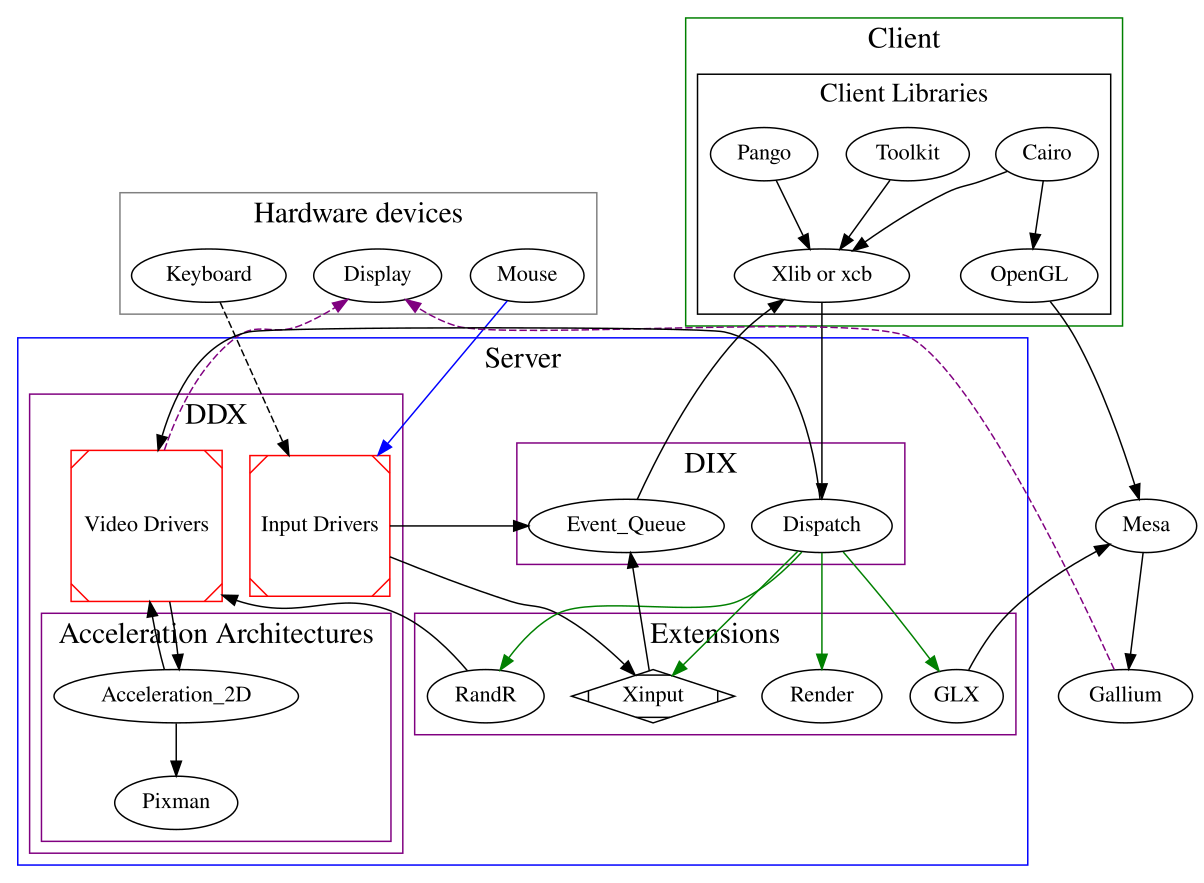
\includegraphics[scale=0.40]{x-1-1.png}
    \caption{X客户端/服务端模型}
    \label{img-1.1.1-1}
\end{figure}

\subsection{X实践}

本节描述X的一些基本组件及其工作原理。这个部分内容很多,有点像大杂烩。推荐的阅读方法是浏览一遍,然后回过头再读一遍。

\subsubsection{通过键盘输入}

X服务执行的任务之一是处理键盘上的输入,并将相应的键事件发送到适当的客户机应用程序。在简单的X配置中,每次只有一个客户端具有“输入焦点”,并且大多数关键事件将发送到该客户端。根据窗口管理器配置,只需将鼠标移动到另一个窗口、单击鼠标、使用热键或操作显示可用客户机的面板,就可以将焦点移动到另一个窗口。具有焦点的客户端通常以某种方式突出显示,以便用户可以知道他们的输入将流向何处。客户端可以使用“抓取”(在本章后面描述)来覆盖向重点客户端发送关键事件的默认交付。



\backmatter
% bibliography, glossary and index would go here.

\end{document}